\section{Spatial Dependence Diagnostics}
\label{sec:si_spatial_diagnostics}

This section consolidates all analyses of spatial autocorrelation across temporal scales. We first describe the covariance structure and testing methodology, then present results for study-period, daily, and hourly data.

\subsection{Covariance Structure}
\label{sec:si_covariance}

To characterize spatial dependence, we assume a covariance function comprised of an exponential term plus a noise term. Defining $d=||x-x'||$, the Euclidean distance between points, this function has the form:
\begin{equation}
 C(d) = \sigma^2 \exp(-d/\ell)+\varepsilon^2
\end{equation}
To fit this model in the original full-year analysis, we first standardize the observations to have mean zero, unit variance. We then fit the covariance function for \city{Dhaka} and \city{Lucknow} using a Gaussian process, assuming a stationary zero mean. Chicago spatial structure is handled with the newer distance-correlation and Moran's $I$ sensitivity outputs because the available Chicago window is a partial-year transferability case rather than a full annual deployment.

Figure~\ref{fig:annual_covariograms} presents the binned empirical variogram across all three networks. In \city{Dhaka} and \city{Lucknow} there is little distance-dependent structure to model at the daily aggregation scale, and the nugget term $\varepsilon^2$ dominates; we therefore expect little benefit from alternative estimators in those two networks. \city{Chicago} shows a different pattern: spatial coupling is detectable in the denser Open Air array, especially at hourly and daily resolution, although the daily pairwise correlations remain uniformly high (median $r=0.970$) and the study-period mean remains a deployed-network estimand rather than an interpolated spatial field.

\begin{figure}[H]
 \centering
 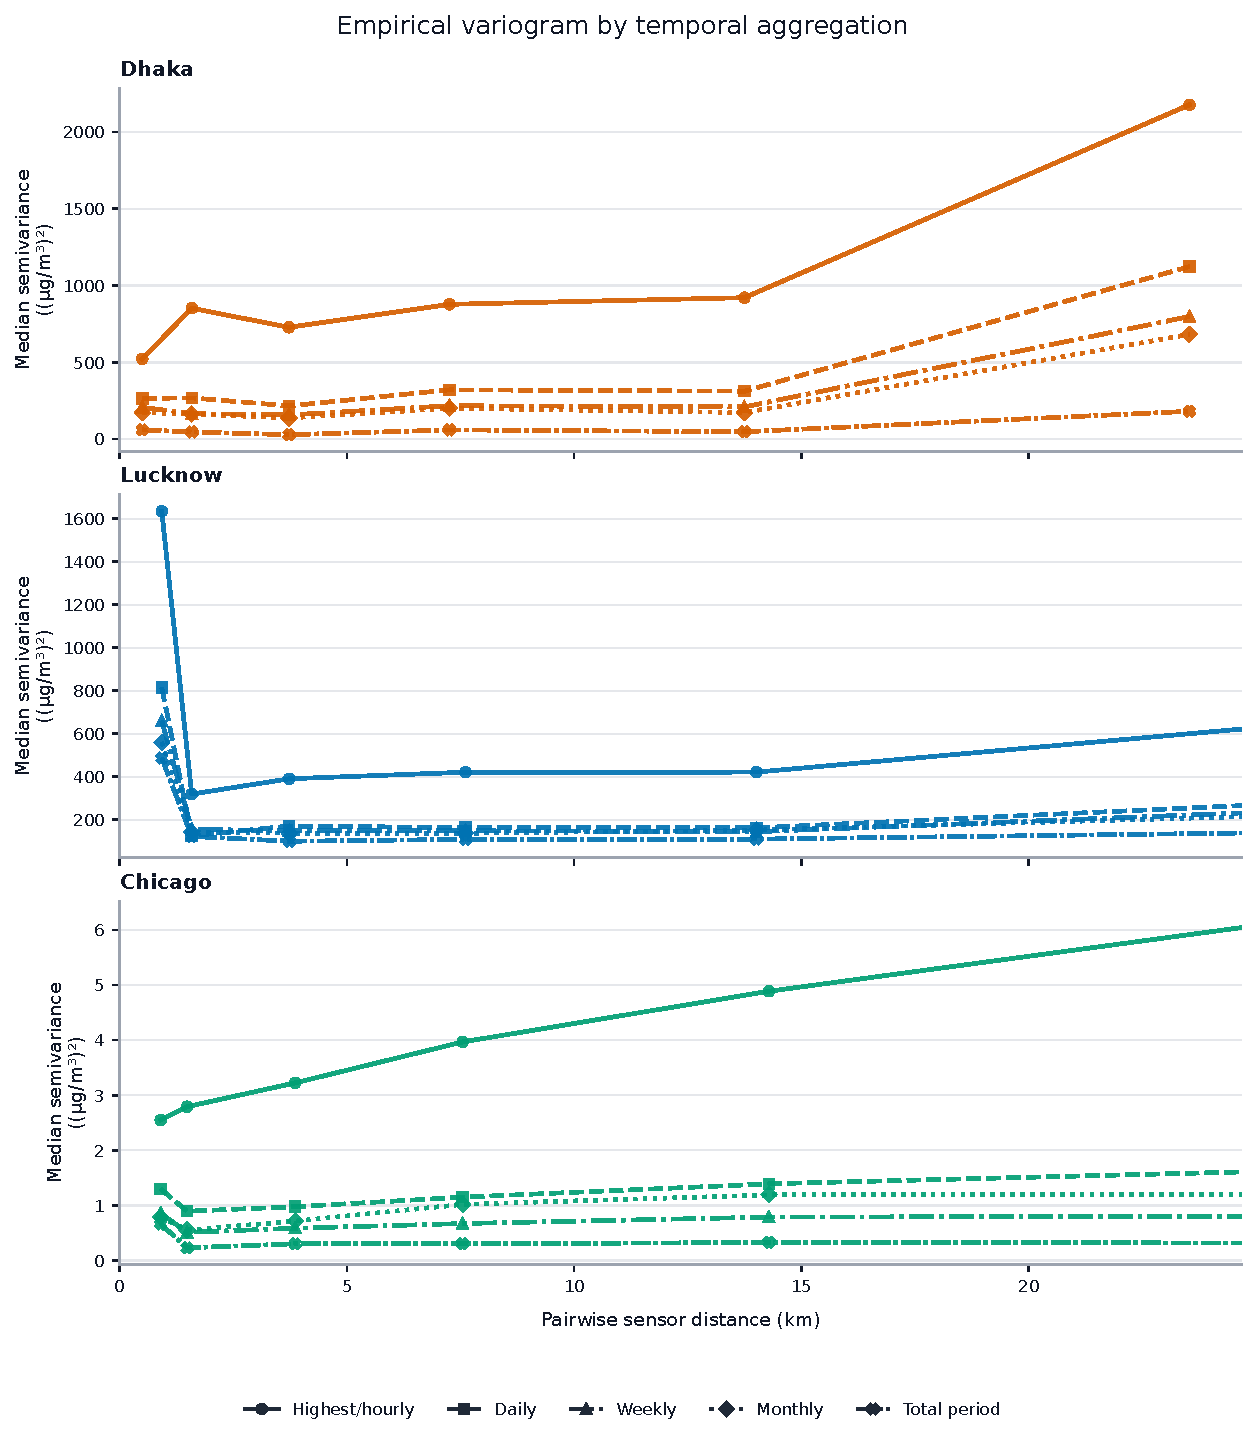
\includegraphics[width=0.95\textwidth]{Plots/Supporting_Information/Figure_SI_2/three_city_empirical_variogram_binned_by_city.pdf}
 \caption{Binned empirical variogram for \city{Dhaka}, \city{Lucknow}, and \city{Chicago}. The variogram quantifies how cross-sensor pair variance grows with separation distance; in \city{Dhaka} and \city{Lucknow} the curve is essentially flat across resolvable distances, consistent with the parametric covariograms showing little or no spatial structure to model at the daily aggregation scale. \city{Chicago} shows a more pronounced increase with distance at the daily scale, reflecting the denser sensor geometry and the stronger Moran's $I$ signal documented in Section~\ref{sec:si_distance_band_sensitivity}.}
 \label{fig:annual_covariograms}
\end{figure}

Figure~\ref{fig:pwod} shows the cumulative distribution of pairwise distances between sensors in all three networks. Because there are few \city{Dhaka} and \city{Lucknow} pairs with less than 5~km separation, we cannot obtain reliable estimates of autocorrelation at shorter distances in those deployments. The \city{Chicago} network has a much higher sensor density (Table~\ref{tab:spatial_support}), giving substantially more short-distance pairs and therefore more power to resolve spatial coupling.

\begin{figure}[H]
 \centering
 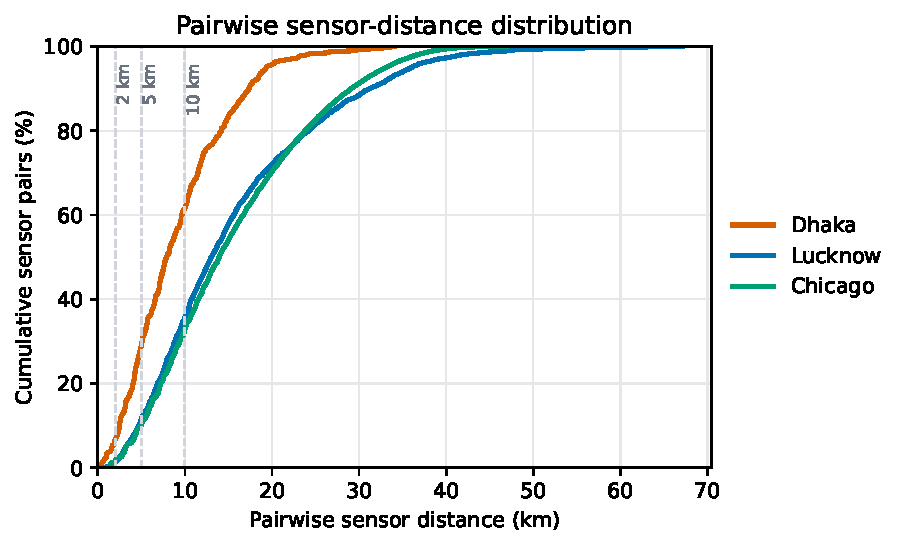
\includegraphics[width=0.95\textwidth]{Plots/Supporting_Information/Figure_SI_3/three_city_cumulative_pairwise_distance.pdf}
 \caption{Cumulative pairwise distance distribution for the \city{Dhaka}, \city{Lucknow}, and \city{Chicago} sensor networks. Vertical reference lines mark 2, 5, and 10~km, the distance bands used in the Moran's $I$ sensitivity analysis. \city{Chicago}'s denser sampling geometry produces far more sensor pairs at short separations.}
 \label{fig:pwod}
\end{figure}

\subsection{Moran's I Method}
\label{sec:si_morans_i}

To test for spatial autocorrelation, we use Moran's $I$ test-statistic with distance-banded weights at 5~km \cite{moran_1950_NotesContinuousStochastic}. This distance threshold is selected based on the pairwise distance distribution (Figure~\ref{fig:pwod}). Formally, Moran's $I$ is defined as:
\begin{equation}
I = \frac{N}{W}\frac{\sum_{i=1}^N\sum_{j=1}^N w_{ij}(y_{i}-\bar{y})(y_j - \bar{y})}{\sum_{i=1}^N (y_i - \bar{y})^2}
\end{equation}
Where $w_{ij}$ defines the weight for pair $ij$, $W=\sum_{i=1}^N \sum_{j=1}^N w_{ij}$. In our networks, we want to determine if there is observable spatial autocorrelation. So, we set $w_{ij} = 1$ for pairs that are less than 5 kilometers apart.

We calculate the Moran's $I$ test statistic by Z-scoring the result, $I$, according to its expected value under the null-hypothesis (i.e., no spatial autocorrelation). This test-statistic is:
\begin{equation}
 z = \frac{I - \mathbb{E}[I]}{\sqrt{\text{VAR[I]}}} \sim \mathcal{N}(0, 1)
\end{equation}
Given this test-statistic, we compare its value to the standard Gaussian curve to determine statistical significance. This test has null hypothesis of complete spatial randomness, $H_0: z=0$, with alternative hypothesis, $H_a:z>0$. If we reject the null hypothesis, spatial autocorrelation is present in the data at the specified distance.

\subsection{Daily and Study-Period Results}
\label{sec:si_spatial_daily_annual}

For daily means under the original 5~km distance-band test, \city{Dhaka} had 9 days (2.5\%) with a statistically significant Moran's $I$ value, assuming a one-sided critical value of $\alpha=0.05$, without correcting for multiple comparisons. For \city{Lucknow}, there were 26 such days (7.1\%). Because this critical value is uncorrected for multiple comparisons, these results show little deviance from what might be expected through random chance. The adaptive k-nearest-neighbor Q-Q diagnostics in Figure~\ref{fig:moran_results} provide the corresponding three-city comparison under a fixed-neighbor geometry: \city{Dhaka} and \city{Lucknow} remain close to the null expectation, whereas \city{Chicago} shows stronger positive departures consistent with its denser sensor geometry.

These results show that, at the spacings observable in our networks, daily spatial autocorrelation is not consistently detectable. Nondetection at the network's spatial resolution does not establish absence of spatial structure; it indicates that local within-day variability dominates any spatially coupled variability when the data are temporally aggregated. There is therefore little to be gained from spatial estimators for the efficiency of deployed-network mean estimation in our networks. It is possible that decreasing the average distance between sensors, or moving to a sub-daily aggregation, would reveal coupling that the present geometry cannot resolve (see Section~\ref{sec:si_hourly_spatial_autocorrelation} and Section~\ref{sec:si_distance_band_sensitivity}).
\begin{figure}[H]
 \centering
 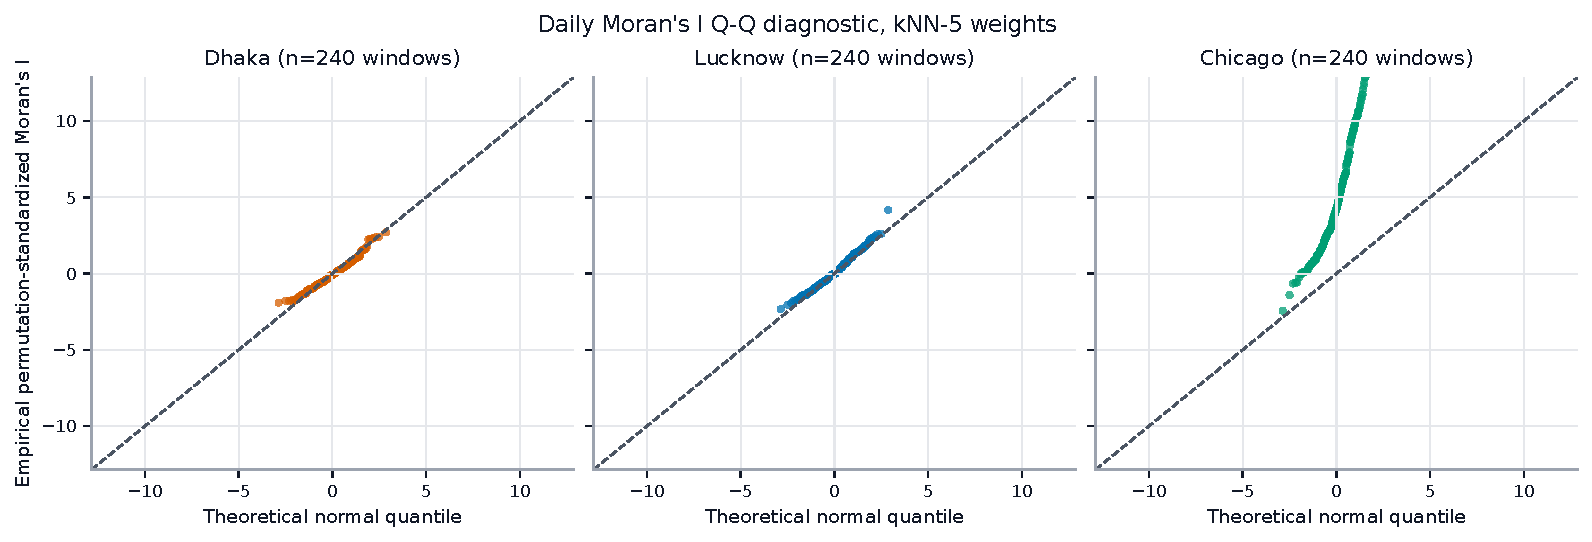
\includegraphics[width=0.95\textwidth]{Plots/Supporting_Information/Figure_SI_4/three_city_daily_morans_i_qq_knn5.pdf}
 \caption{Q-Q plots for daily Moran's $I$ statistics under adaptive k-nearest-neighbor weights ($k=5$) for \city{Dhaka}, \city{Lucknow}, and \city{Chicago}. The x-axis contains theoretical normal quantiles, whereas the y-axis contains the empirical quantiles of standardized Moran's $I$ values. The fixed-neighbor formulation enables a comparable three-city diagnostic despite the much denser \city{Chicago} network.}
 \label{fig:moran_results}
\end{figure}

For study-period means, we obtain Moran's $I = -0.15$ for \city{Dhaka} ($z=-1.4,\;p=0.92$) and $I = -0.08$ for \city{Lucknow} ($z=-0.79,\;p=0.79$) under the original 5~km distance-band test. Under the all-city kNN5 sensitivity screen, the total-period Moran's $I$ values are $-0.060$ in \city{Dhaka}, $-0.040$ in \city{Lucknow}, and 0.063 in \city{Chicago}. We therefore cannot reliably measure spatial autocorrelation to improve study-period mean estimates in the two original full-year networks, while \city{Chicago} again shows a modest positive signal. As above, these results do not establish absence of spatial autocorrelation; they show that spatial autocorrelation tends not to be detectable at length scales observable in \city{Dhaka} and \city{Lucknow} at the 5~km distance band. Indeed, these results imply that accurate neighborhood-level \pmtt\ estimates would require as many sensors as required to obtain accurate deployed-network estimates at this network density --- not until the average inter-sensor distance is small enough to capture genuine spatial coupling will block-kriging produce lower-error estimates than the unweighted mean.

\subsection{Distance-band and resolution sensitivity}\label{sec:si_distance_band_sensitivity}

Because the conclusion above depends on the choice of 5~km distance band, we evaluated Moran's $I$ under a range of bands and weighting schemes: 2~km, 5~km, 10~km, and adaptive nearest-neighbor weights (k = 5). Results are reported in the released analysis outputs. The overall finding is that the daily Moran's $I$ result is qualitatively robust across distance bands in \city{Dhaka} and \city{Lucknow}: significance rates remain near the nominal false-positive rate at all bands examined. \city{Chicago} shows substantively stronger daily spatial autocorrelation under the same tests, with median $k=5$ nearest-neighbor Moran's $I = 0.117$ at the daily scale (compared with $-0.041$ in \city{Dhaka} and $-0.019$ in \city{Lucknow}); the hourly-scale median Moran's $I$ rises further to 0.156 in \city{Chicago}, consistent with the denser sensor network being able to resolve coupling at shorter scales. A binned empirical variogram and binned distance-correlation curve provide complementary views: in particular, the Spearman distance-correlation drops more steeply with distance in \city{Chicago} (daily $\rho = -0.433$) than in \city{Dhaka} (daily $-0.170$) or \city{Lucknow} (daily $-0.250$), reflecting the genuine spatial structure detectable in the denser Chicago array. The variogram and distance-correlation also confirm that inter-sensor pair density is low at short distances in the South Asian networks, limiting power to resolve any short-range coupling that may exist below the 5~km band. The pairwise correlation between sensors at the daily aggregation scale is uniformly high across all three networks (median 0.92 in \city{Dhaka}, 0.96 in \city{Lucknow}, 0.97 in \city{Chicago}), reinforcing the finite-population interpretation: even where short-range spatial structure exists, sensors share a strong common temporal signal at the daily scale.

\subsection{Hourly Autocorrelation}
\label{sec:si_hourly_spatial_autocorrelation}

In the main text, we show that temporal aggregation results in data that exhibit little to no spatial autocorrelation in the two original full-year networks. Here, we demonstrate that hourly data does indeed exhibit spatial autocorrelation. The objective of performing this analysis is to show that spatial autocorrelation exists, and that it should likely be considered when conducting analysis at the sub-daily time-scale. To show this, we perform the same Moran's $I$ analysis as above on the hourly data. We remove any hours for which there were fewer than 20 observations, resulting in 8,239 observations for \city{Dhaka} (94.1\% of hours), and 8,759 observations for \city{Lucknow} (99.9\% of hours). The same k-nearest-neighbor sensitivity screen applied to \city{Chicago} gives a median hourly Moran's $I$ of 0.156, compared with $-0.019$ in \city{Dhaka} and 0.026 in \city{Lucknow}, confirming that the denser Chicago network resolves short-scale spatial coupling more readily.

We summarize the results as Q-Q plots in Figure~\ref{fig:hourly_qq}. The empirical quantiles of the calculated hourly Moran's $I$ statistic demonstrate that the distribution contains values which far exceed what would be expected under the null hypothesis (i.e., that we only obtain high Moran's $I$ values through random chance). This is to be expected, as short-lived meteorology is driving the correlation found in the data at shorter time-scales.

\begin{figure}[H]
 \centering
 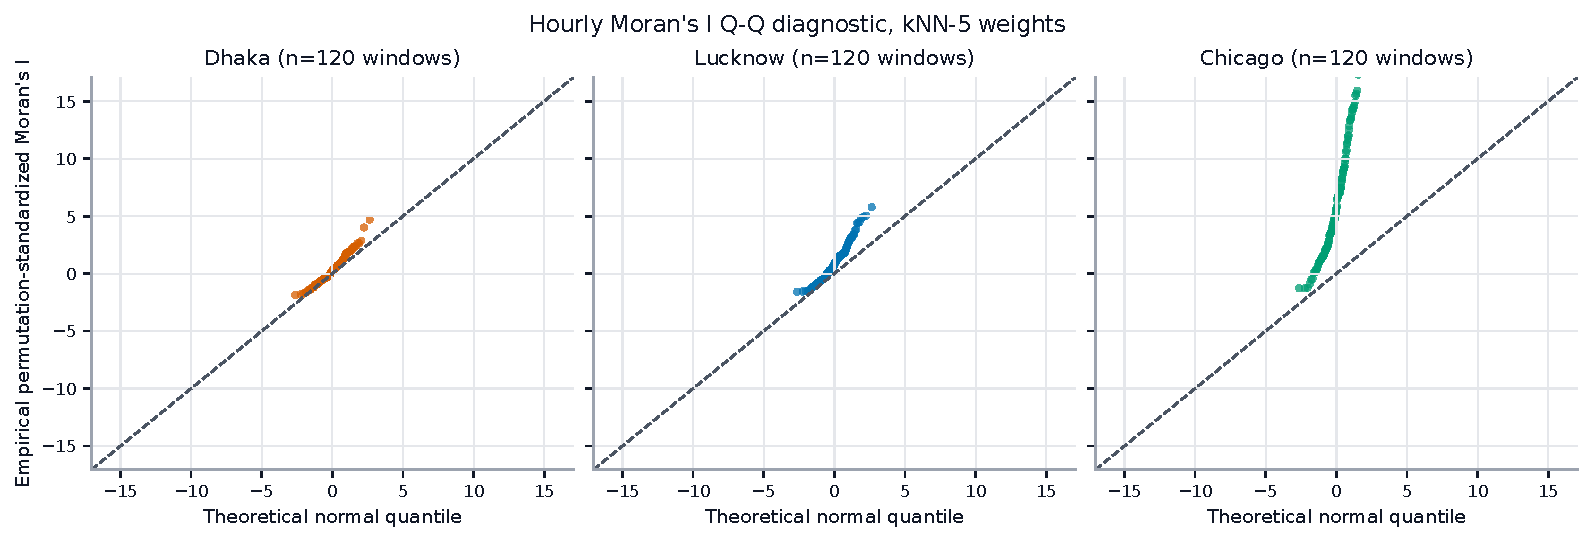
\includegraphics[width=0.95\textwidth]{Plots/Supporting_Information/Figure_SI_5/three_city_hourly_morans_i_qq_knn5.pdf}
 \caption{Q-Q plots for hourly Moran's $I$ statistics under adaptive k-nearest-neighbor weights ($k=5$) for \city{Dhaka}, \city{Lucknow}, and \city{Chicago}. The x-axis contains theoretical normal quantiles, whereas the y-axis contains the empirical quantiles of standardized Moran's $I$ values. The \city{Chicago} panel shows stronger positive departures, consistent with the denser Open Air array resolving short-scale coupling at hourly resolution.}
 \label{fig:hourly_qq}
\end{figure}
